\documentclass[a4paper]{report}
\usepackage[T1]{fontenc}
\usepackage[utf8]{inputenc}
\usepackage{lmodern}
\usepackage{graphicx}
\usepackage[left=3cm,right=3cm,top=3cm,bottom=3cm]{geometry}
\usepackage{eurosym}
\usepackage{fancyhdr}%encabezado y pie de página
\usepackage[colorlinks=true, linkcolor=black, urlcolor=blue]{hyperref}
\setcounter{secnumdepth}{5}
\usepackage[spanish]{babel}
\setcounter{tocdepth}{5}
\usepackage{colortbl}%para colorear tablas
\usepackage{tabularx}
\usepackage{pdfpages}%para incluir documentos pdf
\usepackage{placeins}%para poner barrera y no pasen de secciones los elemntos flotantes
\usepackage{longtable}
\usepackage{multirow} %para juntar varias filas en una tabla

\author{Andoni Martín Reboredo \\ David Ramirez Ambrosi}
\title{\begin{center}
\textbf{\Huge{Práctica 6, Clustering}} \\ 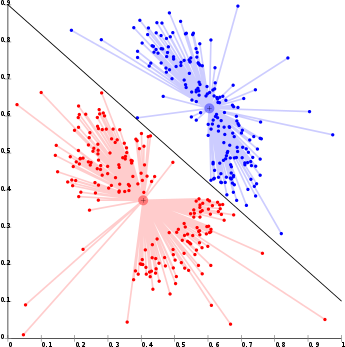
\includegraphics{./Figuras/KMeans-density-data.png}\\  \textbf{Minería de datos}
\end{center}}
\date{\today}



\pagestyle{fancy}
\rhead{
\textbf{Minería de datos} \hfill Práctica 6: Clustering
}

\lhead{}

%colores
\definecolor{azul}{RGB}{0,240,255}
\definecolor{amarillo}{RGB}{255,240,0}
\definecolor{rojo}{RGB}{255,198,198}

%Separación entre párrafos
\setlength{\parskip}{4mm}

\begin{document}
\maketitle

\thispagestyle{empty}%para evitar enumeración de la página de la portada y del índice
\newpage
\tableofcontents%índice
\thispagestyle{empty}
\newpage

\listoffigures%índice de figuras
\thispagestyle{empty}
\newpage

\setcounter{page}{1}%Para reinizar el contador de páginas en la página deseada


\chapter{Introducción}

El presente documento constituye el resultado de la práctica realizada en base a la implementación del algoritmo de clasificación no supervisada \textbf{K-Means clustering}. Este algoritmo trata el agrupamiento de un conjunto de instancias en base a su proximidad con las demás instancias contenidas en el espacio de muestra proporcionado al algoritmo para su ejecución.

Dentro del algoritmo cabe el estudio de diferentes variaciones en los distintos parámetros de que dispone. Nosotros hemos considerado variaciones sobre dos parámetros, el método de cálculo de la distancia entre los distintos elementos que posee el cluster y la inicialización de los distintos clusters. Esta inicialización servirá como base de las sucesivas iteraciones que conforman el algoritmo.

	\section{Clasificación no-supervisada}
	
	La clasificación no supervisada es aquella que se lleva a cabo mediante el estudio de las diversas instancias que conforman el espacio de aplicación del algoritmo sin que estas instancias tengan que estar previamente clasificadas dentro de una clase \cite{clase}.
	
	Se trata de una técnica de exploración de los datos en la que se intentan detectar estas clases desconocidas. Dependiendo de el algoritmo de clasificación utilizado, el número de clases debe o no ser especificado. Por ejemplo, en el algoritmo en que se basa este trabajo debe ser especificado, sin embargo en técnicas de \textbf{clusterig jerárquico} no.
	
	\section{Objetivo}
	
	Esta práctica tiene como objetivo principal la comprensión de los procesos internos que realiza un algoritmo de agrupamiento cualquiera como puede ser el K-Means clustering. El aprendizaje se realizará de forma práctica a través de la implementación del algoritmo K-Means clustering junto con diversas opciones con las que realizar algunos pasos del mismo, como son el uso de métricas o inicializaciones del algoritmo diferentes.	Estas variaciones requieren que el algoritmo sea entendido plenamente para poder hacer contribuciones que tengan utilidad para la realización del proceso.
	
\chapter{Algoritmo}

	\section{K-means, algoritmo principal}
	
	\begin{verbatim}
	inicializar
	divergencia = infinito 
	
	Mientras(numiteraciones <= iteracionesIndicadas AND divergencia < delta)
	{
	    centroides = centroidesNuevos 
	
	    calcularPertenencias
	    centroidesNuevos = calcularNuevosCentroides
		
	    calcularDivergencia(centroidesNuevos) 
	}
	\end{verbatim}
	
	\section{Subrutina inicialización}
		\subsection{Inicialización aleatoria}
			\begin{verbatim}
			Para cada dimensión
			{
			   mientras extraiga una instancia ya evaluada
			   {
			      extraigo una instancia nueva
			   }
			   añado la instancia extraida a las evaluadas
			   establezco la instancia como centroide de un cluster
			}
			\end{verbatim}
		
		\subsection{Pertenencia aleatoria}
			\begin{verbatim}
			Mientras haya instancias que asignar
			{
			   Calculo un número de cluster aleatorio
			   Extraigo la siguiente instancia
			   Añado la instancia al cluster aleatorio
			}
			Calculo los centroides del cluster
			\end{verbatim}
		
		\subsection{División de espacio}
			\begin{verbatim}
			Obtengo los rangos máximos y mínimos de cada subespacio
			Mientras no haya creado k divisiones
			{
			   Mientras no haya establecido todos los atributos(recorrido los subespacios)
			   {
			      Divido el subespacio en K
			      Asigno el centro del subespacio dividido correspondiente al índice del bucle
			   }
			   Añado el centroide resultante de dividir el espacio
			}
			\end{verbatim}
		
		\subsection{Generación aleatoria de codewords}
		\begin{verbatim}
		Obtengo los máximos y mínimos de cada dimensión
		Para cada cluster
		{
		   Evaluo cada dimensión
		   {
		      Calculo un valor aleatorio para ese centroide en esa dimensión
		   }
		   Añado el centroide generado al cluster
		}
		\end{verbatim}
	\section{Subrutina calcularPertenencias}
	
		\begin{verbatim}
		Crear nuevos clusters 
		
		Para cada instancia
		{
		    Para cada centroide
		    {
		        distancia entre la instancia y cada cluster
		        Guardamos los mínimos 
		    }    
		    Para cada centroide obtenido
		        Guardamos la instancia en el cluster correspondiente al centroide
		}
		\end{verbatim}
	
	\section{Subrutina calcularCentroides}
	
		\begin{verbatim}
		Para cada cluster
		
		   Calcular la instancia media
		   
		return nuevosCentroides
		\end{verbatim}
	
	\section{Subrutina calcularDivergencia}
	
		\begin{verbatim}
		Para cada cluster 
		   
		   Calcular la distancia entre el centroide antiguo y el nuevo
		   
		return divergenciaAcumulada
		\end{verbatim}

\chapter{Diseño}

En la figura \ref{fig:clases} se muestra el diagrama de clases final de la aplicación, extraido a partir del código mediante el software \textit{Visual Paradigm}. La especificación de cada uno de los métodos se puede encontrar en la documentación adjunta generada con \textit{Eclipse}, la carpeta doc contiene la \textit{javadoc} generada en forma de \textit{HTMLs} navegables.
	
\begin{figure}[!h]
	\centering
	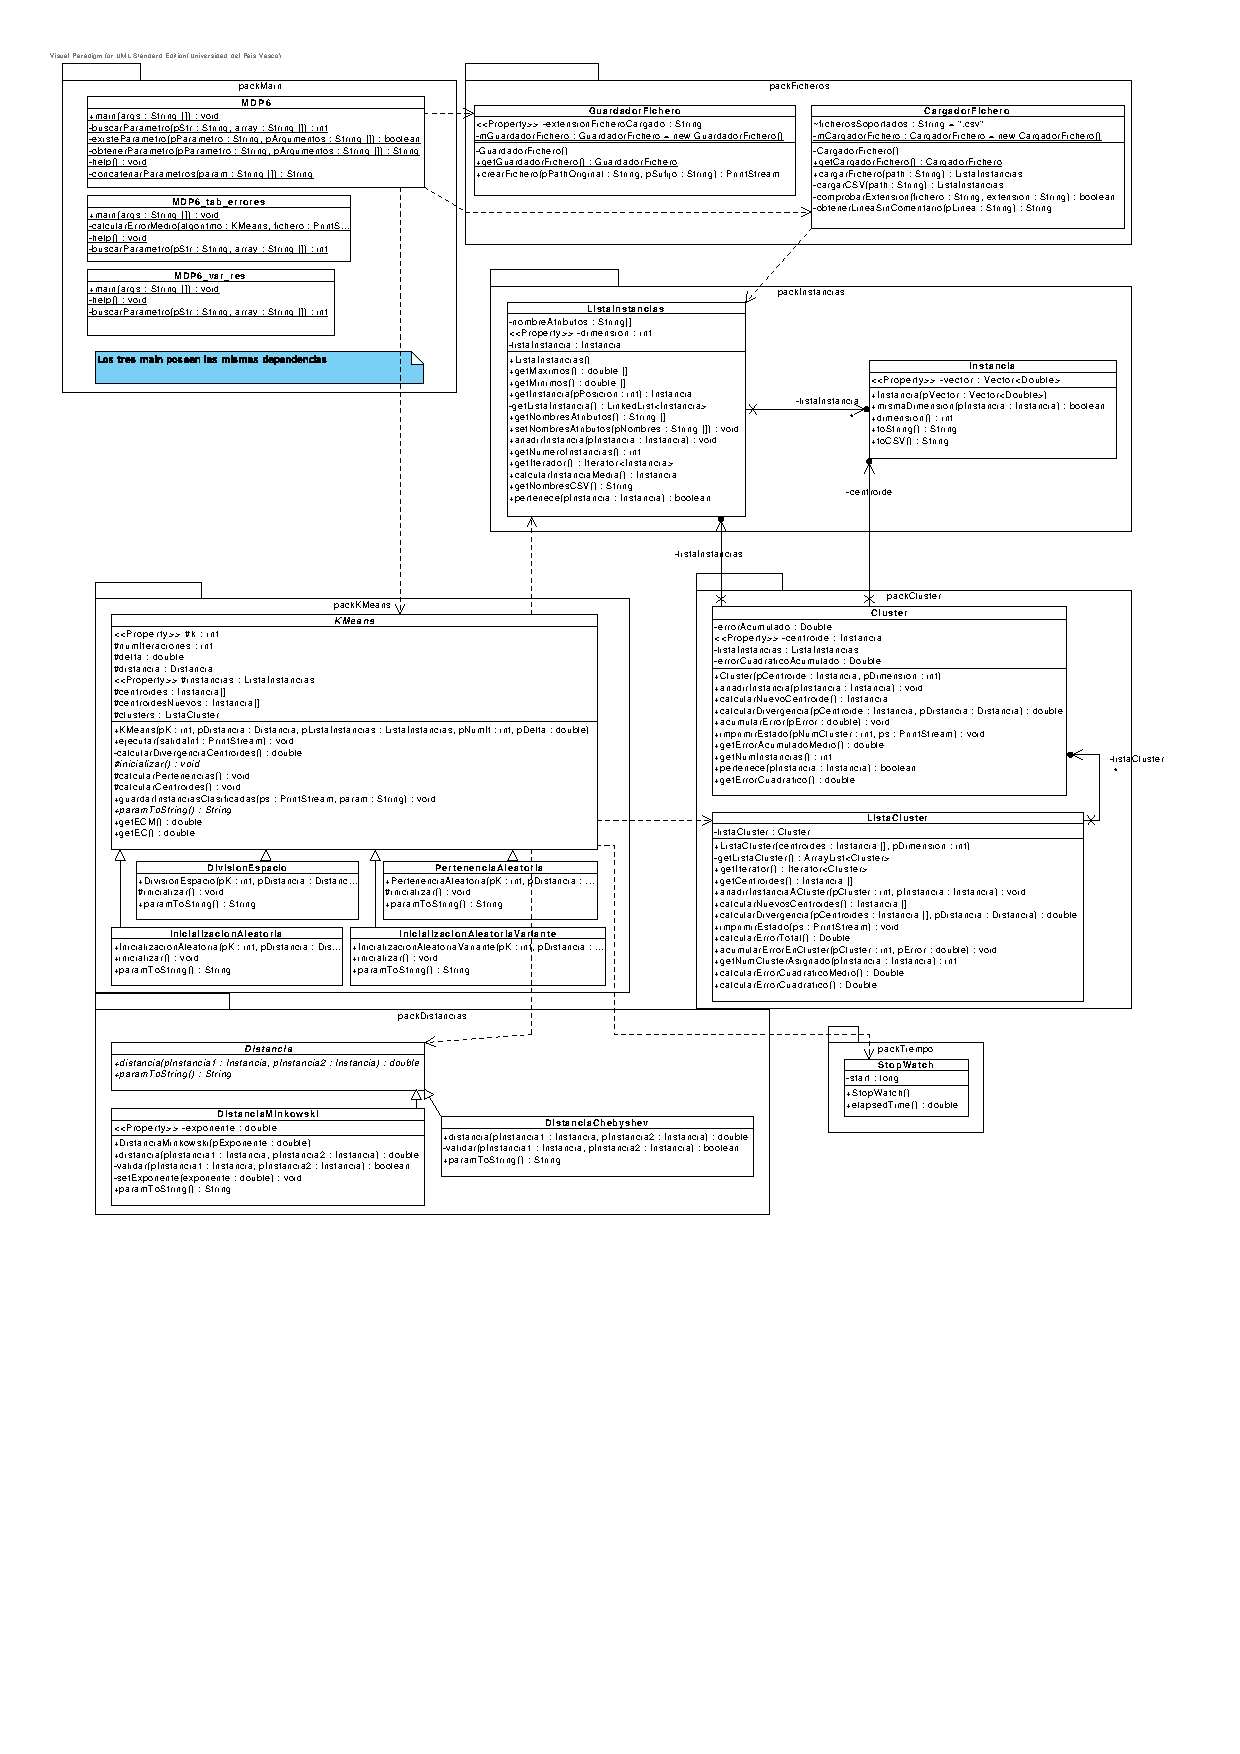
\includegraphics[width=1.1\textwidth, clip=true,trim=1cm 8cm 1.2cm 1cm]{./Figuras/clases.pdf}
	\caption{Diagrama de clases y paquetes}
	\label{fig:clases}
\end{figure}

\chapter{Resultados experimentales}

	\section{Banco de pruebas para la validación de software y resultados}
	
	Para la validación de nuestro software, MDP6, utilizaremos el software Weka usado en la asignatura. Ambos softwares, el propio y Weka, difieren en capacidad y soporte de funciones. Para la realización de pruebas, describimos las capacidades de cada uno de ellos:
	
	
	\begin{center}
		\textbf{MDP6}
	\end{center}
	
	\begin{itemize}
		\item	\textbf{Inicializaciones}. Disponemos de 4 tipos de inicializaciones diferentes:
			\begin{itemize}
			\item	\textbf{Inicialización aleatoria}. Elige al azar k instancias del conjunto de datos para actuar de centroides
			\item	\textbf{Inicialización por petenencia aleatoria}. Por cada instancia, la incluye al azar en uno de los k clusters. Posteriormente se calculan los centroides.
			\item	\textbf{Inicialización por generación aleatoria de centroides}. Se recogen los rangos en que varían los atributos de todas las instancias. Posteriromente se crean k centroides con valores al azar incluidos en los diferentes intervalos identificados.
			\item	\textbf{Inicialización por división de espacio}. Se divide el espacio muestral de acuerdo al número de clusters a crear y se identifican los centroides.
			\end{itemize}
			
		\item	\textbf{Distancias}. Se han implementado dos tipos de métricas capaces de trabajar con el algoritmo
			\begin{itemize}
			\item	\textbf{Distancia Minkowski}. Implementada para cualquier valor del parámetro \textit{m} (siempre que sea un real positivo mayor o igual de 1).
			\item	\textbf{Distancia Chebyshev}.
			\end{itemize}
			
		\item	\textbf{Criterio de parada}. Se ofrece la posibilidad de establecer un límite de iteraciones para la ejecución del algoritmo o bien el uso de un valor a satisfacer para la divergencia entre conjuntos de centroides de dos iteraciones diferentes. También se pueden combinar ambos valores de forma que el primero en satisfacerse determine el fin del algoritmo.
		
		\item	\textbf{Tipos de atributos}. Únicamente se permiten valores numéricos y conocidos para los atributos de las instancias. Todo fichero que vaya a ser cargado debe satisfacer esta condición. No se ofrece funcionalidad como la normalización de atributos.
		
		\item	\textbf{Medidas de calidad}. Como medida del error tras el proceso de clustering se ofrece tanto el \textbf{Error Cuadrático} como el \textbf{Error Cuadrático Medio}.
		
		\item	\textbf{Clasificación de instancias}. Se puede generar un archivo conteniendo las instancias cargadas (en el mismo orden al de entrada) en formato CSV. En este fichero de salida, a cada instancia se le ha añadido un atributo que indica el custer al que finalmente fue asociada tras la ejecución del algoritmo.
		
		\item	\textbf{Repetición de pruebas}. Como se explicará posteriormente, las pruebas realizadas con tipos de inicializaciones que utilicen generación de valores aleatorios no pueden ser repetidas ya que los valores variarán en cada ejecución.
	\end{itemize}
	
	\begin{center}
		\textbf{Weka}
	\end{center}
	
	\begin{itemize}
		\item	\textbf{Inicializaciones}. No ofrece más que un tipo de inicialización.
		
		\item	\textbf{Distancias}. Las distancias disponibles para el agoritmo son Minkowski 1 y Minkowski 2 (Euclídea y Manhattan respectivamente). Además, cada una de estas dos distancias permite normalizarlas.
		
		\item	\textbf{Criterio de parada}. Permite establecer el número máximo de iteraciones que realizará el algoritmo.
		\item	\textbf{Tipos de atributos}. Soporta nominales, numéricos, binarios, unarios, con valores desconocidos o nominales vacíos.
		\item	\textbf{Medidas de calidad}. En el caso de la distancia \textbf{Euclídea}, se ofrece el \textbf{Error Cuadrático} como medida de error. En el caso de la distancia \textbf{Manhathan}, la medida ofrecida es la \textbf{suma de las distancias dentro del cluster}.
		\item	\textbf{Clasificación de instancias}. Tras ejecutar el algoritmo, se puede visualizar el resultado de la agrupación de las instancias y guardarlas en formato \textbf{ARFF} con un atributo más correspondiente al cluster con que la instancia ha sido asociada.
		
		\item	\textbf{Repetición de pruebas}. Weka permite que para una misma semilla (parámetro configurable) los valores generados carezcan de variación, de forma que se puede repetir el mismo experimento una y otra vez para una misma semilla.
	\end{itemize}
	
	Los ficheros utilizados como fuente de instancias han sido \textbf{previamente procesados} con \textit{Weka} para adaptarlos a nuestro software. Se ha procedido a \textbf{eliminar el atributo clase} en aquellos ficheros que la tuvieran y se han guardao las instancias en \textbf{formato CVS}.
	
	Así mismo, en algunos casos ha sido necesario utilizar además un \textbf{procesador de texto} para poder obtener los resultados deseados. También se ha usado el software \textbf{R} para obtener ciertos resultados estadísticos y realizar comparaciones de valores. Para automatizar el proceso de obtención de datos, se han desarrollado programas \textbf{JAVA} extra y se ha utilizado un script del interprete \textbf{BASH}.
	
	Para la representación de resultados se ha utilizado el software \textbf{LibreOffice Calc} y la extensión \textbf{calc2latex} para generar el código Latex de las tablas presentes en este informe.
	
	\subsection{Pruebas realizadas}
	
	Se han realizado tres tipos diferentes de pruebas para comprobar la validez y rendimiento del software desarrollado. En cada una de estas pruebas los indicadores de referencia utilizados han sido:
	
		\begin{itemize}
			\item	\textbf{Medidas de error}. Comparación directa del error generado en el proceso de clustering. Prueba desarrollada en el apartado \ref{rescomparativos}, se utiliza el \textbf{Error Cuadrático} para realizar comparar directamente el software con Weka.
			
			\item	\textbf{Medidas de precisión}. Comparación de la \textbf{precisión} capaz de alcanzar nuestro software con la que Weka es capaz de alcanzar. El proceso se desarrolla y explica en el apartado \ref{resprecision}.
			
			\item	\textbf{Medidas estadísticas}. Uso de medidas como máximo, mínimo, media y varianza de un conjunto de datos para determinar la variabilidad de las repeticiones sucesivas de un determinado experimento con nuestro software. Proceso desarrollado en el apartado \ref{resestadisticos}.
		\end{itemize}
	
	\section{Resultados comparativos}
	\label{rescomparativos}
	
	
	\FloatBarrier
	\section{Clasificación supervisada respecto de otro software de referencia}
	\label{resprecision}
		
	\section{Variabilidad de los resultados}
	\label{resestadisticos}

	
	\section{Análisis crítico y discusión de resultados}
	
	\section{Rendimiento del software}

\chapter{Conclusiones}

	\section{Motivación para la realización de \textit{Clustering}}
	
	Explorar un conjunto de instancias con el objetivo de 
	
	\section{Conclusiones de los resultados}
	
	\section{Conclusiones generales}
	
	El tiempo invertido en el proyecto ha sido mucho mayor conforme se acercaba la fecha de entrega. Debemos mejorar en organización, especialmente al principio de la práctica, donde un diseño poco especificado con ciertas cosas \textit{"en el aire"} nos llevaron a diseñar al implementar.
	
	También el hecho de probar y perfeccionar el funcionamiento de \textbf{todo} el código antes de comenzar con la extracción de resultados experimentales nos limitó en el análisis de los mismos y en la retroalimentación del algoritmo implementado.
	
	Resumiendo, hay que mejorar la planificación, dividir el proyecto en partes para poder mejorarlo incrementalmente.
	
	Pese a los problemas, la solución implementada ofrece una variedad bastante amplia de parámetros posibles a utilizar, teniendo 4 tipos de inicialización, dos métricas diferentes - en el caso de la métrica Minkowski ofrece otro parámetro más que variar- y la posibilidad de controlar el número de iteraciones tanto por la especificación de un maximo de vueltas, como por la especificación del margen de variación que se debe alcanzar hasta dar por válidos los centroides identificados.
	
	\section{Propuestas de mejora}
	
	La entrada a nuestro programa es un factor un tanto restrictivo en el sentido de que el único tipo de fichero soportado es el \textbf{CSV}. Inicialmente, la intención era implementar también la carga de ficheros \textbf{ARFF}, que no ha sido posible hacerla por falta de planificación principalmente.
	
	En cuanto a inicializaciones, hemos implementado 4 tipos diferentes. De los tres, el correspondiente a la división de espacio es el que más puede mejorar, ya que para su implementación no hemos llegado a consultar bibliografía extra.
	
	La \textbf{estimación del error} es otro apartado en el que nos ha quedado duda, ya que el proceso de cálculo utilizado no ha sido el mismo que el usado por Weka y nos dificultaba la comparación de ambos algoritmos utilizando esta medida.
	
	Otra restricción se da por el tipo de datos tratados, el algoritmo solo es capaz de lidiar con atributos de tipo numérico, siendo imposible realizar la carga de instancias que contengan valores no numéricos. De hecho, algunos de los ficheros han tenido que ser preprocesados para poder trabajar con ellos.
	
	Otro problema ya arrastrado de trabajos anteriores, es la \textbf{presentación de resultados}. No en cuanto a la información presentada, sino a como se presentan concretamente los\textbf{ valores reales}, que deberían ser redondeados a, por ejemplo, 3 decimales. Esto permitiría que los informes generados sean más fáciles de leer e interpretar.

%Bibliografía

\newpage
\bibliographystyle{plain}

\bibliography{mdp6}

\newpage


\chapter{Valoración subjetiva}
	
	\section*{Alcance de objetivos}
	
	\section*{Utilidad de la tarea}
	
	\section*{Dificultad}
	
	\section*{Tiempo de trabajo}
	
	\section*{Sugerencias de mejora}
	
	\section*{Críticas}

\end{document}